%%==========================
%% chapter01.tex for TJU Master Thesis
%% based on CASthesis
%% modified by charlie.yaha@gmail.com
%% version: 0.1alpha
%% Encoding: UTF-8
%% last update: Dec 5th, 2010
%%==================================================

%\bibliographystyle{TJU} %[此处用于每章都生产参考文献]


\newcommand{\citeA}[2]{\citeauthor{#1}\cite{#1}}

\chapter{绪~论}

\section{研究背景及意义}
地下介质普遍具有衰减性,其衰减性通常用品质因子$Q$来表征。地震衰减对地表反射地震数据有非常重要的影响,
主要表现在如下两方面。首先,地震衰减会减弱地震波的振幅从而减低地震成像的分辨率;其次,地震衰减会使
地震波的相位变形以及速度频散,以致于地震成像不聚焦、位置错位。图(\ref{fig:spectral}a)对比了在同一时刻接收的
非衰减的地震波(蓝色)和在$Q=30$的介质中传播的地震波的波形。从图中可以看出,衰减介质中传播地震波
的振幅被极大程度的吸收衰减。由于地震衰减导致速度频散,高频成分的地震波具有更快的传播速度,所以
两列波具有不同的到达时。同时地震衰减会改造地震波的相位,从而破坏地震波波形的对称性。
图(\ref{fig:spectral}b)对应地展示了图(\ref{fig:spectral}a)中两种波的振幅谱。
从图中可以明显看出,高频成分的衰减要
远远严重于低频成分,这也是造成图(\ref{fig:spectral}a)中振幅强衰减的主要原因。

\begin{figure*}[!htbp]
        \centering
        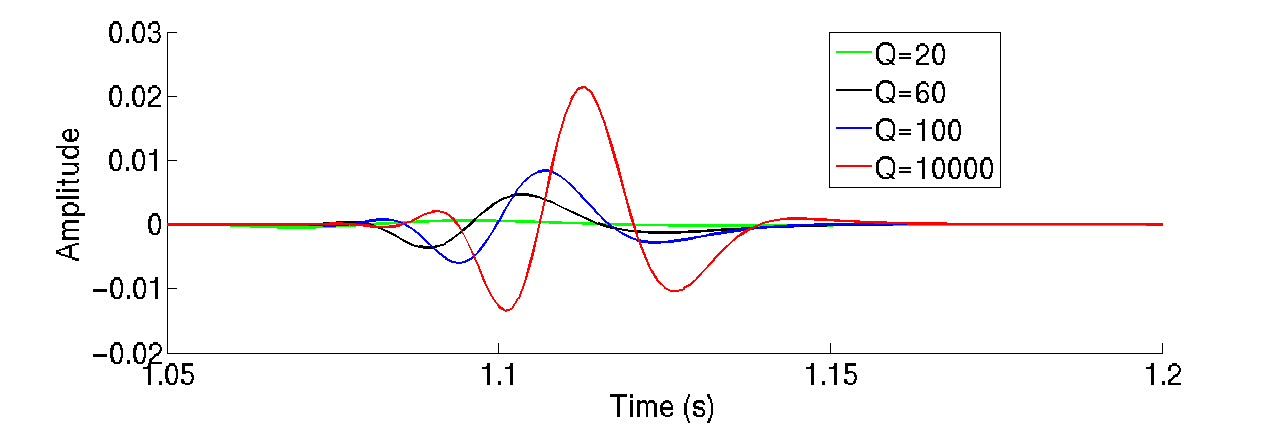
\includegraphics[width=0.9\linewidth]{figure/spectral}
        \fcaption{地震波在声介质和粘声介质($Q=30$)中传播的数值模拟实验:
	(a)地震波波形图;(b)对应的振幅谱。}{1D example to numerically illustrate the attenuation 
	impacts on the amplitudes spectra and phase of propagating wave: (a) the 
	non-attenuated waveform (blue curve) and the attenuated waveform (red curve); (b) the 
	corresponding amplitude spectral. }[展示地震衰减效应的一维数值实验]
        \label{fig:spectral}
\end{figure*}

在地震波偏移成像中,如果不补偿$Q$的效应,同样会影响地震成像的质量。地震衰减通过吸收地震波的
高频成分和改造地震波的相位来降低地震波成像的质量。图(\ref{fig:qrtm}c)展示了用准确$Q$补偿的
逆时偏移($Q$-RTM)成像结果。像被精确地成在了深度为800m的地方,并且像在强衰减区域下面有
均衡的能量。图(\ref{fig:qrtm}d)是没用$Q$补偿的RTM结果。由于频散的速度在成像中
没有得到校正,成像的位置要稍微浅于800m,并且在强衰减区域下方成像能量弱。在地震勘探过程,
不考虑$Q$的影响可能会导致地震解释不准确,甚至导致钻井错位。

\begin{figure*}[!htbp]
        \centering
        \includegraphics[width=0.9\linewidth]{figure/rtm_no.pdf}
		\fcaption{衰减对成像的影响实验:(a) 速度模型; (b)$Q$模型;(c)$Q$-RTM成像结果;
		(d)RTM成像结果}{ (a) The velocity model. (b) The $Q$ model.
		(c) The migrated image with a correct $Q$ compensation. (d) The migrated image without
		$Q$ compensation.}[衰减对成像的影响实验]
        \label{fig:qrtm}
\end{figure*}

在实际勘探中,气云/气包区的成像、储层识别和解释都面临巨大的挑战。气云/包区通常包含极低的
$Q$值,这种强烈的衰减会吸收深部同相轴的能量,在储层的上方造成成像阴影区,严重影响地震
解释的准确性。可靠的$Q$模型不仅可以提高成像的质量,而且可以更好解释振幅随偏移距变化
(AVO)和各向异性这两种依赖于偏移距的效应。正确的AVO和各向异性
解释可以提高油气勘探的成功率。另外,$Q$模型可以作为一个表征岩石和流体属性的参数,
例如在稀疏井控制下,可以用$Q$模型来检测岩性的边界(\citeA{desgupta.clark:1998},)。
衰减量级是一个直接刻画储层的油气物理参数,例如可以直接利用$Q$模型来确定储层含气/油
的饱和度(\citeA{winkler.nur:1982},)。在油气开发过程中,衰减模型还可以用来指示储层裂缝的方位
(\citeA{maultzsch.chapman:2007}, ,\citeA{clark.benson:2009},)以及监控流体的运移能力,
帮助优化注水过程(\citeA{macrides.kanasewich:1987},)。
因此,在油气勘探开发过程中,定量地评估衰减效应,构建一个可靠的衰减($Q$)模型是非常重要的。
本文主要的工作就是通过反射全波形反演来定量估计地震本征衰减$Q$模型。

\vspace{0.5cm}
\section{国内外研究现状}

国内外学者对$Q$模型估计做了大量的研究工作,其中大部分工作都是在数据域完成。数据域的
反演方法可大致分为两类:基于高频近似的射线层析类和基于波动方程的波形反演类。

射线类方法中,\citeA{brzostowski.mcmechan:1992},首先用观测数据振幅与震源振幅比值的对数作为输入数据来
实现$Q$层析成像。但是除了吸收衰减外,影响振幅的因素还有很多如几何扩散、透射/反射损失、
散射损失等。为了区分衰减引起的振幅损失,\citeA{quan.harris:1997},将观测数据和计算数据间质心
频率的移动作为匹配准则,用射线层析方程来更新$Q$模型。\citeA{hu.liu:2011},用震源的振幅谱作为
拟合函数来处理地震数据频谱非对称性的影响,并用多指数盒状约束法来消除非地震本征衰减的影响。
质心频率移动类的方法相对于振幅匹配类方法对噪音不敏感,所以更适合于处理实际数据。
射线类方法计算效率高,处理简单横向变化的地质构造有很好的效果。但是在上覆介质复杂时,
地震波存在多路径,射线类方法由于不能处理多路径情况而造成误差。波动类层析方法可以
有效的解决多路径问题。

波形反演(FWI)是一种通过求解波动方程来恢复地下介质参数的反演迭代方法(\citeA{tarantola:1984},)。
传统的FWI主要是用于反演声波速度。
\vspace{0.5cm}
\section{本文研究内容}


















